%% ===== 5 Results =====
\section{Results}
\label{sec:results}

% [27/10] "columns do not sum to 49" không đúng hẳn (ở Bảng 8, cột chia theo legacy cộng lại bằng tổng của oracle đó);
% nói chung cho mọi hình và bảng. "use several migration kinds" thành "involve".
% [28/10] Tầng I3 thành mục 5.5.
Counts below refer to the 49 papers of the main corpus; the two cross-language equivalence-detection papers (I3) \new{are reported in Section~\ref{sec:i3}}. A paper can use several oracles and \new{involve} several migration kinds, so \new{the counts in a figure or table can add up to more than 49}.

%% ---------------------------------------------------------------------
\subsection{Corpus overview}
\label{sec:overview}

% [27/10] Số kiểm từ coding.csv và Bảng 2 (năm, tỉ lệ, track, kiểu, vai trò LLM). "research-track" thành "come from the
% research track"; bỏ dấu phẩy trước "and" như phần còn lại của bài.
The corpus grows quickly: \new{8 papers are from 2024, 14 from 2025 and 27 from 2026}\hcrev{, or 0.68\%, 0.98\% and 1.45\% of the papers scanned in each year (Table~\ref{tab:search}). The 2024 share may be slightly low, since 61 ICSE~2024 papers had no abstract and were matched on their titles only.}

\new{Most papers come from the research track (28); the others come from} industry/SEIP (\new{9}), journal-first (5), NIER (3)\new{, posters (2), demonstrations (1) and Ideas, Visions and Reflections (IVR, 1). We call the NIER, IVR, demonstration and poster papers short papers.} Translation between languages dominates (XL, 33 papers), followed by library migration (LIB, 12), version migration (VER, 3), framework migration (FW, 3) and dialect translation (DIA, 2); 5 papers migrate legacy systems\hcrev{, as defined in Section~\ref{sec:background}}. Rust is a target language in 13 papers. The LLM is the proposed technique in 32 papers, the evaluated subject in 9 \new{and both in 4}; in the remaining 4 it is \hcrev{only a baseline (3,} \new{2} \hcrev{of which propose a smaller neural model) or part of the evaluation tooling (1)}.

%% ---------------------------------------------------------------------
% [28/10] Tiêu đề dạng câu hỏi thành cụm danh từ như các RQ khác.
\subsection{RQ1: \new{Oracles in use}}
\label{sec:rq1}

% [27/10] Thêm câu 14/49 so output với chương trình gốc (Related Work trỏ tới đây; 14 = O-f, hai bài O-g đều có O-f).
% Câu về cách đếm trỏ về quy tắc ở 4.5. [28/10] "compare outputs with it" thành "execute it to compare behavior": bộ chấm
% LLM của WCA4Z cũng đọc mã COBOL gốc (đã kiểm), nên chỉ đúng khi nói chạy chương trình gốc. "execute" như Abstract và RQ4.
Compilation and existing tests dominate; formal verification\hcrev{, LLM-generated tests} and LLM judges are rare (Figure~\ref{fig:oracle-freq}). \new{Every migration has the original program as a reference, yet only 14 papers (29\%) execute it to compare behavior, all by differential testing. Because an oracle is counted whenever a paper reports its result (Section~\ref{sec:extraction}),} \hcrev{the counts record which oracles} \new{the} \hcrev{papers use, not which ones their conclusions rest on.}

\begin{figure}[t]
  \centering
  %% Figure: oracle frequency in the 49 main-corpus papers (mapping/4_coding/coding.csv;
%% mapping/analysis/recompute.py prints the same numbers).
%% A paper can use several oracles, so bars do not sum to 49.
%% To change a number, edit both the bar value and its label [n (p%)].
%% Revised 26 Oct 2026 after review: TRAVEL, PtrTrans, ReCodeAgent and MBTA
%% recoded, and CAST gains O-b under the compilation rule (option B);
%% bars sorted by count again.
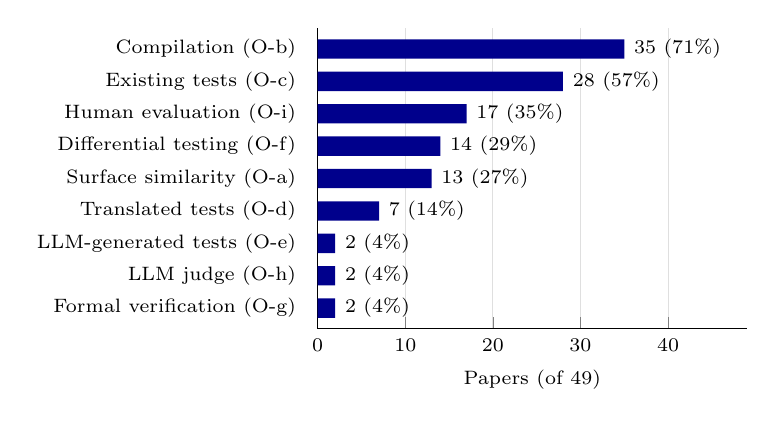
\begin{tikzpicture}
\begin{axis}[
  xbar, width=0.58\columnwidth, height=5.4cm, xmin=0, xmax=49, y dir=reverse,
  ytick=data, symbolic y coords={ob,oc,oi,of,oa,od,oe,oh,og},
  yticklabels={{Compilation (O-b)},{Existing tests (O-c)},{Human evaluation (O-i)},{Differential testing (O-f)},{Surface similarity (O-a)},{Translated tests (O-d)},{LLM-generated tests (O-e)},{LLM judge (O-h)},{Formal verification (O-g)}},
  yticklabel style={font=\scriptsize}, xticklabel style={font=\scriptsize},
  xtick={0,10,20,30,40}, xmajorgrids, grid style={gray!25}, axis lines*=left, ytick style={draw=none},
  bar width=7pt, enlarge y limits=0.08,
  point meta=explicit symbolic, nodes near coords, nodes near coords style={font=\scriptsize, anchor=west},
  xlabel={\scriptsize Papers (of 49)}, clip=false,
]
  \addplot[fill=blue!55!black, draw=none] coordinates {(35,ob) [35 (71\%)] (28,oc) [28 (57\%)] (17,oi) [17 (35\%)] (14,of) [14 (29\%)] (13,oa) [13 (27\%)] (7,od) [7 (14\%)] (2,oe) [2 (4\%)] (2,oh) [2 (4\%)] (2,og) [2 (4\%)]};
\end{axis}
\end{tikzpicture}
  % [27/10] O-b 35 theo phương án B. Chú thích gộp ba câu ngắn thành câu định nghĩa cột; thêm "bars sum to more than 49".
  \caption{\revtag \new{Number of main-corpus papers (of 49) that report a result for each oracle on the final outputs. A paper can use several oracles, so the bars sum to more than 49.}}
  \Description{Horizontal bar chart. Compilation 35 papers (71\%), existing tests 28 (57\%), human evaluation 17 (35\%), differential testing 14 (29\%), surface similarity 13 (27\%), translated tests 7 (14\%), LLM-generated tests 2 (4\%), LLM judge 2 (4\%), formal verification 2 (4\%).}
  \label{fig:oracle-freq}
\end{figure}

% [27/10] Số theo phương án B (16/18/6; bỏ \TODO V2). "9 use one" thay bằng "(40 of 49)" vì 9 bài này khác 9 bài ở câu sau. Câu
% 5/28 chuyển xuống đoạn Bảng 6. Câu năm bài một oracle bỏ vế lặp "does not run the code"; Collaboration còn báo "success rate"
% nhưng không nói kiểm bằng gì, nên chỉ mã O-a (đã kiểm với bài gốc). "executes the code" như Abstract và RQ4.
Most papers \new{(40 of 49)} combine oracles: \new{16 use two, 18 use three and} 6 use four or more, up to \hcrev{five in RustAssure~\cite{rustassure}.} Nine papers use no oracle that executes \new{the} code (none of O-c to O-f) \new{and} judge outputs by compilation, similarity, a human or an LLM. \hcrev{Five} \new{of them} \hcrev{rely on a single oracle}\new{: BLEU or CodeBLEU in two}~\cite{vimpt,collaboration}\new{, an LLM judge in one}~\cite{wca4z} \new{and human judgment in two}~\cite{pig,pli}.

\begin{added}
% [27/10] Phương án B: 22 thành 23, 6 thành 5. Câu 5/28 từ đoạn trên, bỏ "their code must compile to run" (sai: BDUpdater đích
% JavaScript; UniTrans, TransAgent, InterTrans có đích Python). Câu differential testing nêu rõ 14 bài O-f, đủ 4 + 9 + 1 (RustAssure
% dùng O-d). "also run" thành "also use": RustAssure chỉ có một phép so ký hiệu, mã cả O-f lẫn O-g.
Table~\ref{tab:cooc} shows which oracles are combined. Compilation accompanies most other oracles\new{: 23 of the 28 papers with existing tests and} \hcrev{12 of the 17} \new{with human evaluation also use it. The remaining 5 of the 28 report no compile rate, so for compiled targets a translation that fails to compile cannot be told apart from one that compiles but fails the tests.} \new{Of the 14 papers that use differential testing, only 4 combine it with existing tests; in 9 it is the only test-based oracle, and the last pairs it with translated tests.} \new{Both papers with formal verification also use differential testing, in VERT~\cite{vert} as a step before model checking and in RustAssure~\cite{rustassure} as part of the same symbolic check.}
\end{added}

\begin{table}[t]
  \centering
  \caption{\addedtag\revtag Oracle combinations in the main corpus. Each cell counts the papers that use both oracles; the diagonal gives the papers that use each oracle.}
  \label{tab:cooc}
  % [27/10] Phương án B: CAST (O-a, O-b, O-c) thêm O-b, nên 6 thành 7, 34 thành 35, 22 thành 23. Đã đối chiếu mọi ô với coding.csv.
  \footnotesize
  \setlength{\tabcolsep}{3.5pt}
  \begin{tabular}{@{}lrrrrrrrrr@{}}
    \toprule
        & O-a & O-b & O-c & O-d & O-e & O-f & O-g & O-h & O-i \\
    \midrule
    O-a & \hcrev{13} &  &  &  &  &  &  &  &  \\
    O-b & \new{7} & \new{35} &  &  &  &  &  &  &  \\
    O-c & \hcrev{7} & \new{23} & 28 &  &  &  &  &  &  \\
    O-d & \hcrev{0} & 7 & 5 & 7 &  &  &  &  &  \\
    O-e & \hcrev{1} & \hcrev{1} & \hcrev{1} & \hcrev{0} & \hcrev{2} &  &  &  &  \\
    O-f & \hcrev{1} & \hcrev{12} & \hcrev{4} & 3 & \hcrev{0} & \hcrev{14} &  &  &  \\
    O-g & 0 & 2 & 0 & 1 & 0 & 2 & 2 &  &  \\
    O-h & \hcrev{0} & \hcrev{1} & \hcrev{0} & \hcrev{0} & \hcrev{0} & \hcrev{0} & 0 & \hcrev{2} &  \\
    O-i & \hcrev{4} & \hcrev{12} & \hcrev{6} & \hcrev{3} & \hcrev{0} & \hcrev{5} & 1 & \hcrev{1} & \hcrev{17} \\
    \bottomrule
  \end{tabular}
\end{table}

%% ---------------------------------------------------------------------
\subsection{RQ2: \new{Ground-truth origin and context of use}}
\label{sec:rq2}

% [27/10] Tiêu đề theo RQ2 ở Intro. Phần ground truth (đoạn và bảng) chuyển lên trước phần ngữ cảnh, theo thứ tự của RQ2 và Method.
\begin{added}
% [27/10] Tách ba đoạn (O-c; O-d, O-e; O-f); "test-based" như Background. "client project" sai với FreshBrew (VER). Nói rõ
% IntentTester chỉ di trú test (vì sao 5 với 4); bài thuộc cả hai nhóm O-d đã có ở chú thích bảng. Bỏ câu LLM-written tests vì
% trùng Background, nên bỏ cả "Only". Java-to-ArkTS, GUIMigrator và hai nguồn input của ReCodeAgent đã kiểm với bài gốc.
\paragraph{Where the ground truth comes from.} Table~\ref{tab:origin} breaks down the four \new{test-based} oracles by the origin of their ground truth\hcrev{; we do not code the origin of the other oracles}. Existing tests split almost evenly \new{by who wrote them: benchmark builders in 14 papers, a real project's developers in 12 and both in 2~\cite{dgir,recodeagent}}. \hcrev{Among the 14 LIB and VER papers, 7 use existing tests, and 6 of these 7} \new{run the project's own suite on the migrated code}\hcrev{~\cite{pylibmig,byam,fruntke,bdupdater,googlemig,freshbrew}.} In translation between languages, benchmark tests are more common: 12 papers, against \new{6} with project suites and \new{2} with both.

% [28/10] Câu đầu đổi thứ tự cho khỏi hai câu liền mở bằng "In N of".
\new{The system under evaluation produces the translated tests in 5 of the 7 papers that use them. In 4 of these the same system also translates the code, and} a translation error can therefore affect the code and its tests alike; in IntentTester\new{, which migrates only tests,} the migrated tests are themselves the output under evaluation\hcrev{, so a} \new{passing test shows only that its assertions hold} \hcrev{on the target library, not that} \new{they} \hcrev{still check what the original test checked}\new{~\cite{intenttester}. The authors translate tests by hand for their own evaluation in 3 of the 7 papers~\cite{lostintranslation,rustassure,recodeagent}.} \new{Two} \hcrev{papers use LLM-generated tests in the sense of Table~\ref{tab:oracles}, where the expected outputs come from an LLM or a specification: one derives its tests from the same specification it uses to generate the code~\cite{ipmodern}, and one does not} \new{state the origin of its expected outputs~\cite{transagent}, so by the rule in Section~\ref{sec:extraction} we code it as O-e}.

\new{Differential testing always compares outputs with the original program, so for this oracle we code the origin of its inputs:} fuzzing, property-based testing or symbolic execution in 5 papers, existing tests or benchmark data in 3 \new{and an LLM} in \hcrev{3~\cite{prognosticator,travel,recodeagent}}\new{. Java-to-ArkTS runs both versions on curated samples~\cite{arkts}, GUIMigrator compares the rendered screens before and after migration~\cite{guimigrator} and 2 papers do not describe their inputs; ReCodeAgent has two input origins}\hcrev{~\cite{recodeagent}}.
\end{added}

\begin{table}[t]
  \centering
  % [27/10] "test-based" như Background; nêu rõ O-f mã nguồn input. Bỏ "Origin is coded only…" vì đoạn văn đã nói. Hai câu
  % tổng hàng gộp lại vì cùng là ReCodeAgent (d:S, d:H; f:L, f:U).
  \caption{\addedtag\revtag \new{Origin of the ground truth of test-based oracles in the main corpus; for differential testing, origin of the inputs.} Per-paper codes are in Appendix~\ref{app:primary}. \new{One paper~\cite{recodeagent} appears in two O-d rows and in two O-f rows, so the O-d rows sum to 8 and the O-f rows to 15.}}
  \label{tab:origin}
  \small
  \begin{tabular}{@{}P{0.8\linewidth}r@{}}
    \toprule
    Oracle and origin & Papers \\
    \midrule
    \multicolumn{2}{@{}l}{\textit{O-c Existing tests (28)}} \\
    \quad Built for a benchmark (curated problems, reference translations) & 14 \\
    \quad A real project's own test suite & 12 \\
    \quad Both & 2 \\
    \multicolumn{2}{@{}l}{\textit{O-d Translated tests (7)}} \\
    \quad Translated by the system under evaluation & 5 \\
    \quad Translated by hand by the authors & 3 \\
    \multicolumn{2}{@{}l}{\textit{O-e LLM-generated tests (\hcrev{2})}} \\
    \quad Derived from the specification that also generates the code & 1 \\
    \quad \new{Origin} of expected outputs not stated & 1 \\
    \multicolumn{2}{@{}l}{\textit{O-f Differential testing (\hcrev{14})}} \\
    \quad Inputs from fuzzing, property-based testing or symbolic execution & 5 \\
    \quad Inputs from existing tests or benchmark data & 3 \\
    \quad Inputs generated by an LLM & \hcrev{3} \\
    \quad Curated samples or rendered screens & 2 \\
    \quad Inputs not described & 2 \\
    \bottomrule
  \end{tabular}
\end{table}

% [27/10] "Most groups are small" quá tay: chỉ 5 trong 14 nhóm có ≤ 5 bài. Đổi chỗ gạch journal-first và 2026 theo thứ tự ngữ cảnh.
% Câu mở đoạn bỏ dấu hai chấm và "four contexts" (đã có ở Method).
\paragraph{\new{How oracle use differs by context.}} \new{Table~\ref{tab:context} splits the corpus by legacy status, migration kind, track and year. The legacy, VER, FW, DIA and journal-first groups have five papers or fewer each, so} \hcrev{patterns in} \new{them} \hcrev{are illustrative only.}

\begin{table*}[t]
  \centering
  % [27/10] Phương án B: CAST (XL, không legacy, journal-first, 2026) thêm O-b, nên cột O-b: 33→34, 22→23, 4→5, 19→20. Đã đối
  % chiếu mọi ô với coding.csv. Trỏ Appendix như Bảng 7 (để kiểm các ý chéo nhóm ở các gạch). Thêm câu về 4 bài có hai loại
  % di trú (n cộng lại 53); dòng short papers ghi tên như 5.1.
  \caption{\revtag Oracle use by context. Each cell counts papers in the group that use the oracle; $n$ is the group size. \new{Per-paper codes are in Appendix~\ref{app:primary}. A paper with two migration kinds counts in both rows, so the migration-kind rows sum to 53. IVR: Ideas, Visions and Reflections.}}
  \label{tab:context}
  \small
  \begin{tabular}{@{}lrrrrrrrrrr@{}}
    \toprule
    Group & $n$ & O-a & O-b & O-c & O-d & O-e & O-f & O-g & O-h & O-i \\
    \midrule
    Legacy                    & 5 & 0 & 1 & 0 & 0 & 1 & 2 & 0 & 1 & 1 \\
    Not legacy                & 44 & \hcrev{13} & \new{34} & 28 & 7 & \hcrev{1} & \hcrev{12} & 2 & \hcrev{1} & \hcrev{16} \\
    \midrule
    XL                        & 33 & \hcrev{7} & \new{23} & 20 & 6 & \hcrev{2} & \hcrev{11} & 2 & \hcrev{1} & \hcrev{6} \\
    LIB                       & 12 & 4 & 9 & 6 & 2 & 0 & 1 & 0 & 1 & 9 \\
    VER                       & 3 & 1 & 2 & 1 & 0 & 0 & 1 & 0 & 0 & 1 \\
    FW                        & 3 & 1 & 3 & 1 & 0 & 1 & 1 & 0 & 0 & 1 \\
    DIA                       & 2 & 1 & 1 & 0 & 0 & 0 & 1 & 0 & 0 & 2 \\
    \midrule
    Research                  & 28 & \hcrev{8} & 19 & 15 & 6 & \hcrev{1} & 8 & 2 & \hcrev{1} & \hcrev{13} \\
    Industry/SEIP             & 9 & 2 & 7 & 5 & 1 & \hcrev{1} & \hcrev{3} & 0 & 1 & 2 \\
    \new{Short:} NIER, IVR, demo, poster & 7 & 2 & 4 & 3 & 0 & 0 & 2 & 0 & 0 & 2 \\
    Journal-first             & 5 & 1 & \new{5} & 5 & 0 & 0 & 1 & 0 & 0 & 0 \\
    \midrule
    2024                      & 8 & 3 & \hcrev{5} & 5 & 1 & 0 & 2 & 0 & 0 & 1 \\
    2025                      & 14 & 3 & 10 & 8 & 3 & 0 & 4 & 2 & 0 & 6 \\
    2026                      & 27 & \hcrev{7} & \new{20} & 15 & 3 & \hcrev{2} & \hcrev{8} & 0 & \hcrev{2} & \hcrev{10} \\
    \bottomrule
  \end{tabular}
\end{table*}

% [27/10] Legacy: TRAVEL, DGIR, PtrTrans cũng gọi mã C là legacy (đã kiểm bài gốc), nên "the three papers" và "2 of 8" sai.
% LIB: nói rõ 6 trong 9 bài có chạy code; bỏ câu "No LIB paper…" (trùng gạch ô trống). Bỏ "final-output" vì mọi oracle được
% mã đều chấm đầu ra cuối (4.5). Ô trống: "Other" vì hai ô đã nêu ở trên; "test-suite" sai với DIA (có O-f); 1.3 lớn nhất là
% legacy × O-a (5 × 13/49).
\begin{itemize}
  % [28/10] "several ... most of them" thành "at least 4": nhiều bài C sang Rust dùng chữ legacy (cả C2SaferRust, PtrTrans), nên chỉ khẳng định 4 bài đã kiểm.
  \item \textbf{\new{No legacy paper uses existing tests.}} Two of the 5 legacy papers run the original system as a differential oracle~\cite{kcobagent,coboljava}, one generates tests with an LLM from an extracted specification~\cite{ipmodern}, one uses an LLM judge~\cite{wca4z} and one \new{compares the generated Java with the expected code by hand}~\cite{pli}. \hcrev{This is the one empty cell that chance does not easily explain: with 28 of the 49 papers using existing tests, about 3 legacy papers would be expected to use them. With} \new{5} \hcrev{papers, all in the industry/SEIP or NIER tracks, legacy cannot be separated from track}\new{. The result also} \hcrev{depends on our definition:} \new{the legacy flag does not cover C, yet at least 4 C-to-Rust papers call their C sources legacy and use existing tests~\cite{evoc2rust,smartc2rust,travel,dgir}.}
  % [28/10] "these nine" thành "these 9" như "the other 3" trong cùng câu.
  \item \textbf{\hcrev{Library migration often includes a human check.}} \new{Nine of the 12} LIB papers include human evaluation, against \hcrev{6} of 33 XL papers\new{. Six of these 9 also execute the code, and the other 3 judge behavior without executing it}\hcrev{~\cite{pig,depupgrade,rulesynth}. Several human checks cover only part of the outputs, such as a 20\% sample of the patches that pass the tests~\cite{fruntke} or the 24 cases that have a developer's fix~\cite{bdupdater}.}
  \item \textbf{\hcrev{Both formal-verification papers target Rust}}~\cite{rustassure,vert}\hcrev{; with two papers, this is an observation rather than a pattern.}
  \item \hcrev{\textbf{All 5 journal-first papers use existing tests}, and none uses human evaluation.}
  \item \textbf{\hcrev{LLM-based} \new{oracles} \hcrev{appear only in 2026.}} \hcrev{The 2 papers with LLM-generated tests~\cite{ipmodern,transagent} and the 2 with LLM judges~\cite{depupgrade,wca4z} are all from 2026. Earlier papers use LLM-generated tests only inside the technique~\cite{unitrans,collaboration}, and with four papers the timing may be chance.}
  \item \textbf{\new{Other zero cells}} \new{include legacy with O-a, O-d or O-g; LIB with O-e or O-g; DIA with O-c, O-d or O-e; and short papers with O-d, O-e, O-g or O-h.} \new{If oracle use did not depend on the group, each of these cells would hold at most 1.3 papers}\hcrev{, so an empty cell says little on its own.}
\end{itemize}

%% ---------------------------------------------------------------------
\subsection{RQ3: Threats to oracle reliability}
\label{sec:rq3}

% [28/10] Viết lại đoạn mở của bản cyan: bỏ phép cộng 18+8-2+9; nêu đủ 7 trong 40 bài không có số riêng cho từng oracle trên cùng
% output, chia theo lý do (thêm C2SaferRust và MSA; biểu đồ của TransGraph không ghi số).
\paragraph{Oracle disagreement.} \new{Thirty-three of the 40 papers that combine oracles (Section~\ref{sec:rq1}) report separate numbers for two or more of them on the same outputs. The other 7 do not: four apply the oracles as successive checks and report only the final outcome~\cite{byam,c2saferrust,ipmodern,googlemig}, one gives a number for a single oracle~\cite{deepmodelx}, one applies them to different outputs~\cite{msa} and one shows the per-oracle results only in a chart without values~\cite{transgraph}.}

% [28/10] Đếm xong 33 bài trước khi phân tích hình và bảng: 18 ở Hình 3, 6 chỉ có ở Bảng 9, 9 bài còn lại gom theo lý do (đối chiếu bài
% gốc). "show other disagreements" thành "compare other oracles" vì Bảng 9 có cả bài không lệch (TransAgent); "have no such pair of
% rates" thành "fit neither the figure nor the table" vì Bảng 9 có cả số đếm và điểm. Python library migration chỉ chạy test trên 25
% trong 314 output, nên viết "no behavioral pass rate on the same outputs".
\new{Of the 33, 18 give both a compile rate (or the pass rate of another well-formedness check) and a behavioral rate (Figure~\ref{fig:compile-gap}), and 6 more compare other oracles (Table~\ref{tab:disagree}). The remaining 9 fit neither the figure nor the table: they count compile errors or bugs rather than outputs~\cite{smartc2rust,prognosticator}, pool failures over several models~\cite{lostintranslation,rustrepotrans}, measure compilation and equivalence in different units~\cite{rustassure} or report similarity scores or manual judgments with no behavioral pass rate on the same outputs~\cite{codeplan,guimigrator,rulesynth,pylibmig}.}

% [28/10] Gộp chú thích hai bản. Thêm: DepUpgrade (62/119) và IntentTester (1.996/2.776) báo tỷ lệ hành vi trên bản biên dịch được,
% Hình 3 tính lại trên mọi output (62/123, 1.996/3.257); các dòng khác lấy số của bài hoặc tính từ số đếm. Nhãn trong hình là số
% nguyên (đã đối chiếu file trên Overleaf), nên bỏ câu "two decimal places". "Mapping CSV" ghi rõ là gói replication
% (figure3_compile_vs_behavior.csv). DGIR thành DepTrans như bài gốc (DGIR chỉ là khung suy luận). Nhãn DepUpgrade thành
% "(GPT-5.4)" để mọi ngoặc trên hình đều là cấu hình; cách chấm của từng bài ghi ở câu áp chót.
\begin{figure}[t]
  \centering
  %% Figure: compile rate vs behavioral pass rate in the 18 papers that report both
%% for the same outputs (recount 25/10/2026, revised after an independent check;
%% sheet "Mã hoá tổng hợp", column "Nhiều oracle trên cùng output", group "Hình 3";
%% numbers from field 6 of "Trích xuất (nháp)", checked against the papers).
%% Each row: (compile rate, behavioral pass rate) as reported or computed from the fractions
%% below; rows sorted by gap.
%% Fractions used: DepUpgrade 119/123 and 62/123 (equivalent patches over all
%% tasks); Fruntke & Krinke 40/65 and 12/65; VERT 539/569 and 295/569;
%% IntentTester 2,776/3,257 and 1,996/3,257; RISE 136/143 and 124/143;
%% Translation Tag Team 274/350 and 253/350; BatFix 605/698 and 567/698.
%% If a value changes, edit it here AND the gap label on the right.
%% [28/10] Dòng 1: DGIR thành DepTrans như bài gốc (DGIR chỉ là khung suy luận). Dòng 2: AlphaTrans 24.50% (chỉ GS)
%% thành 25.14%, tỷ lệ tương đương chức năng ở abstract của bài (GS + M1 All); khoảng cách vẫn là 74. Đã đối chiếu
%% 18 dòng với bài gốc; nhãn khoảng cách là số nguyên, khớp hiệu đã làm tròn. Nhãn DepUpgrade "(judged equivalent)"
%% thành "(GPT-5.4)" để mọi ngoặc đều là cấu hình (cách chấm đã ghi ở chú thích hình).
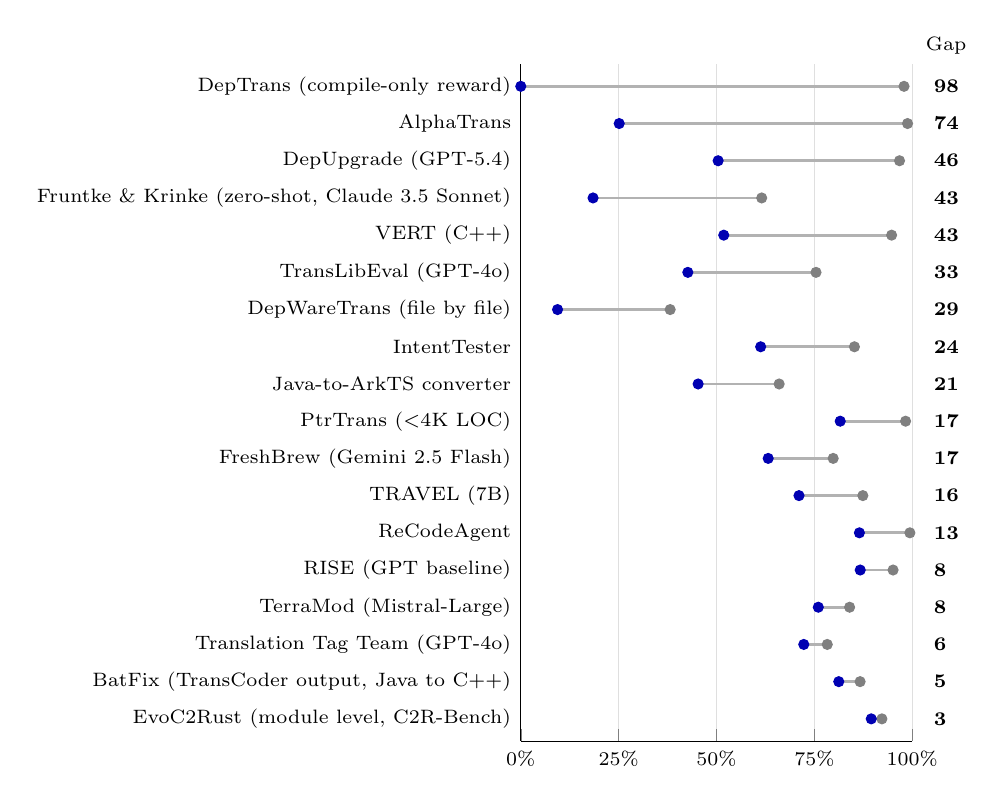
\begin{tikzpicture}
\begin{axis}[
  scale only axis, width=0.41\columnwidth, height=8.6cm,
  xmin=0, xmax=100, ymin=0.4, ymax=18.6, y dir=reverse,
  ytick={1,...,18}, yticklabels={{DepTrans (compile-only reward)},{AlphaTrans},{DepUpgrade (GPT-5.4)},{Fruntke \& Krinke (zero-shot, Claude 3.5 Sonnet)},{VERT (C++)},{TransLibEval (GPT-4o)},{DepWareTrans (file by file)},{IntentTester},{Java-to-ArkTS converter},{PtrTrans ($<$4K LOC)},{FreshBrew (Gemini 2.5 Flash)},{TRAVEL (7B)},{ReCodeAgent},{RISE (GPT baseline)},{TerraMod (Mistral-Large)},{Translation Tag Team (GPT-4o)},{BatFix (TransCoder output, Java to C++)},{EvoC2Rust (module level, C2R-Bench)}},
  yticklabel style={font=\scriptsize}, xticklabel style={font=\scriptsize},
  xtick={0,25,50,75,100}, xticklabel={\pgfmathprintnumber{\tick}\%},
  xmajorgrids, grid style={gray!25}, axis lines*=left, ytick style={draw=none},
  clip=false,
]
  \draw[gray!60, line width=1pt] (axis cs:0.00,1) -- (axis cs:97.90,1);
  \draw[gray!60, line width=1pt] (axis cs:25.14,2) -- (axis cs:98.80,2);
  \draw[gray!60, line width=1pt] (axis cs:50.41,3) -- (axis cs:96.75,3);
  \draw[gray!60, line width=1pt] (axis cs:18.46,4) -- (axis cs:61.54,4);
  \draw[gray!60, line width=1pt] (axis cs:51.85,5) -- (axis cs:94.73,5);
  \draw[gray!60, line width=1pt] (axis cs:42.67,6) -- (axis cs:75.42,6);
  \draw[gray!60, line width=1pt] (axis cs:9.39,7) -- (axis cs:38.16,7);
  \draw[gray!60, line width=1pt] (axis cs:61.28,8) -- (axis cs:85.23,8);
  \draw[gray!60, line width=1pt] (axis cs:45.30,9) -- (axis cs:66.00,9);
  \draw[gray!60, line width=1pt] (axis cs:81.60,10) -- (axis cs:98.30,10);
  \draw[gray!60, line width=1pt] (axis cs:63.20,11) -- (axis cs:79.80,11);
  \draw[gray!60, line width=1pt] (axis cs:71.07,12) -- (axis cs:87.38,12);
  \draw[gray!60, line width=1pt] (axis cs:86.50,13) -- (axis cs:99.40,13);
  \draw[gray!60, line width=1pt] (axis cs:86.71,14) -- (axis cs:95.10,14);
  \draw[gray!60, line width=1pt] (axis cs:76.00,15) -- (axis cs:84.00,15);
  \draw[gray!60, line width=1pt] (axis cs:72.29,16) -- (axis cs:78.29,16);
  \draw[gray!60, line width=1pt] (axis cs:81.23,17) -- (axis cs:86.68,17);
  \draw[gray!60, line width=1pt] (axis cs:89.53,18) -- (axis cs:92.25,18);
  \addplot[only marks, mark=*, mark size=1.8pt, color=gray] coordinates {(97.90,1) (98.80,2) (96.75,3) (61.54,4) (94.73,5) (75.42,6) (38.16,7) (85.23,8) (66.00,9) (98.30,10) (79.80,11) (87.38,12) (99.40,13) (95.10,14) (84.00,15) (78.29,16) (86.68,17) (92.25,18)};
  \addplot[only marks, mark=*, mark size=1.8pt, color=blue!70!black] coordinates {(0.00,1) (25.14,2) (50.41,3) (18.46,4) (51.85,5) (42.67,6) (9.39,7) (61.28,8) (45.30,9) (81.60,10) (63.20,11) (71.07,12) (86.50,13) (86.71,14) (76.00,15) (72.29,16) (81.23,17) (89.53,18)};
  \node[anchor=west, font=\scriptsize\bfseries] at (axis cs:103,1) {98};
  \node[anchor=west, font=\scriptsize\bfseries] at (axis cs:103,2) {74};
  \node[anchor=west, font=\scriptsize\bfseries] at (axis cs:103,3) {46};
  \node[anchor=west, font=\scriptsize\bfseries] at (axis cs:103,4) {43};
  \node[anchor=west, font=\scriptsize\bfseries] at (axis cs:103,5) {43};
  \node[anchor=west, font=\scriptsize\bfseries] at (axis cs:103,6) {33};
  \node[anchor=west, font=\scriptsize\bfseries] at (axis cs:103,7) {29};
  \node[anchor=west, font=\scriptsize\bfseries] at (axis cs:103,8) {24};
  \node[anchor=west, font=\scriptsize\bfseries] at (axis cs:103,9) {21};
  \node[anchor=west, font=\scriptsize\bfseries] at (axis cs:103,10) {17};
  \node[anchor=west, font=\scriptsize\bfseries] at (axis cs:103,11) {17};
  \node[anchor=west, font=\scriptsize\bfseries] at (axis cs:103,12) {16};
  \node[anchor=west, font=\scriptsize\bfseries] at (axis cs:103,13) {13};
  \node[anchor=west, font=\scriptsize\bfseries] at (axis cs:103,14) {8};
  \node[anchor=west, font=\scriptsize\bfseries] at (axis cs:103,15) {8};
  \node[anchor=west, font=\scriptsize\bfseries] at (axis cs:103,16) {6};
  \node[anchor=west, font=\scriptsize\bfseries] at (axis cs:103,17) {5};
  \node[anchor=west, font=\scriptsize\bfseries] at (axis cs:103,18) {3};
  \node[anchor=west, font=\scriptsize] at (axis cs:101,-0.1) {Gap};
\end{axis}
\end{tikzpicture}
  \caption{\new{Share of outputs that pass compilation or another well-formedness check (gray) and share that pass the behavioral check (blue) in the 18 papers that report both for the same outputs. Numbers on the right give the gap in percentage points. Each row shows the configuration in parentheses or otherwise the paper's own system; the RISE and DepWareTrans rows are baselines, the DepTrans row is an ablation and the BatFix row shows the translations before repair. Rates are as reported or computed from reported counts, except that DepUpgrade and IntentTester report the behavioral rate over the outputs that compile and we recompute it over all outputs. The behavioral check differs by paper (DepUpgrade uses human review, IntentTester's outputs are tests and ReCodeAgent counts passing tests rather than programs), so a gap is meaningful only within its row. The replication package lists each configuration and where the paper reports it.}}
  \Description{Dot plot with one row per paper. Gaps range from 98 percentage points for the DepTrans ablation (97.9\% compile, 0\% correct) to 3 percentage points for EvoC2Rust (92.25\% versus 89.53\%).}
  \label{fig:compile-gap}
\end{figure}

% [28/10] Thay đoạn cyan và câu "Other disagreements involve…": giữ cách viết của bản cyan (nhận định rồi dẫn chứng), gộp ý MBTA
% của bản cyan vào câu áp chót, giữ khoảng 3 đến 98 điểm của đoạn mở bản gốc. Không nhắc lại số đã có trong hình và bảng. Các số đếm
% (13/18, 4/5, cả 4 bài, MBTA 168) đã kiểm với bài gốc; chi tiết ở hai file CSV của Hình 3 và Bảng 9 trên GitHub.
\new{Figure~\ref{fig:compile-gap} and Table~\ref{tab:disagree} show the limits of compilation, surface similarity and testing. Compilation accepts many outputs that fail the behavioral check: the behavioral rate trails the compile rate by 3 to 98 percentage points across the 18 configurations in Figure~\ref{fig:compile-gap}, and by more than 10 points in 13 of them. Similarity scores do not reliably reflect test results. Exact match rejects most translations that pass the tests in both papers that report the two~\cite{unitrans,cast}. In 4 of the 5 papers that report a similarity score next to a pass rate on the same outputs, the score ranks at least one pair of systems or settings in the opposite order to the pass rate~\cite{unitrans,cast,terramod,dgir}. For TerraMod and DepTrans, a variant that passes fewer tests even scores higher than the proposed system~\cite{terramod,dgir}. Tests and fuzzing also accept outputs that a further check rejects. All 4 papers that apply such a check find these outputs in every setting they report~\cite{bdupdater,codehints,fruntke,vert}. How many fail it differs greatly: one of the 24 BDUpdater updates, against 16 of the 23 Code hints candidates without code hints. In MBTA, TransCoder reaches perfect CA on 168 programs yet mistranslates at least one mutant of each~\cite{mbta}. A translation that passes all its tests therefore does not show that the translator handles small changes to the program. The rows of Table~\ref{tab:disagree} use different measures and cannot be pooled.}

% [28/10] Thêm cột Outputs judged; Result chỉ còn số theo thứ tự oracle. Bảng nay gồm mọi bài của ba nhóm (thêm DepTrans, Fruntke &
% Krinke), bài có hai cấu hình đáng so thì hai dòng. "disagreements" thành "comparisons": ở TransAgent, CodeBLEU xếp cùng thứ tự với CA
% ở cả 6 hướng dịch. CAST là 4 hướng dịch (2 cặp ngôn ngữ), không phải 4 cặp. Số đã kiểm với bài gốc: UniTrans, TransAgent T2; CAST T1;
% TerraMod, Code hints, Fruntke & Krinke, VERT T1; DepTrans T5 (cột TOTAL); BDUpdater T8; MBTA mục RQ2.
\begin{table*}[t]
  \centering
    \caption{Other oracle \new{comparisons} on the same outputs\new{. Each group includes all main-corpus papers of its kind. Outputs judged: one or two of several settings per paper. Results follow the order of the oracles compared, with scores on each paper's own scale. Four papers also appear in Figure~\ref{fig:compile-gap}. CA: computational accuracy, the share of outputs that pass the tests. MTS: mutation-based translation score, the share of a program's mutants that the translator gets wrong}.}
  \label{tab:disagree}
  \small
  \begin{tabular}{@{}P{0.15\linewidth} P{0.29\linewidth} P{0.27\linewidth} P{0.20\linewidth}@{}}
    \toprule
    Paper & \new{Outputs judged} & Oracles compared & Result \\
    \midrule
    \multicolumn{4}{@{}l}{\new{\textit{Similarity next to a pass rate}}} \\
    UniTrans~\cite{unitrans} & \new{LLaMA-33B, 1-shot, average of four translation directions} & Tests (CA) vs exact match & \new{47.63\% vs 9.16\%} \\
     & \new{TransCoder-ST, average of four translation directions} & & \new{52.15\% vs 7.70\%} \\
    CAST~\cite{cast} & \new{Qwen2.5-72B, 1-shot, average of four translation directions} & Tests (CA) vs exact match & \new{68.36\% vs 15.67\%} \\
     & \new{LLaMA3-70B, 1-shot, average of four translation directions} & & \new{65.67\% vs 16.76\%} \\
    TransAgent~\cite{transagent} & \new{TransCoder (a baseline), Python to Java} & Tests (CA) vs CodeBLEU & \new{2.4\% vs 40.1} \\
     & \new{TransAgent, Python to Java} & & \new{89.5\% vs 69.8} \\
    TerraMod~\cite{terramod} & \new{LLaMA-4-Maverick without migration context (Base)} & Execution (Pass@1) vs CrystalBLEU & \new{44\% vs 0.78} \\
     & \new{LLaMA-4-Maverick with migration context (TerraMod)} & & \new{76\% vs 0.66} \\
    \new{DepTrans~\cite{dgir}} & \new{RAST-7B, compile and test reward weights 1:1, both benchmarks} & \new{Tests (CA) vs CodeBLEU} & \new{43.5\% vs 65.4} \\
     & \new{RAST-7B, compile and test reward weights 1:2 (ablation), both benchmarks} & & \new{40.8\% vs 66.5} \\
    \multicolumn{4}{@{}l}{\new{\textit{Further check on outputs that pass tests or fuzzing}}} \\
    BDUpdater~\cite{bdupdater} & \new{GPT-4.1, 24 updates} & Existing tests vs developer's fix & \new{24 vs 23} \\
    Code hints~\cite{codehints} & \new{Symbolic engine, deprecated methods with code hints} & Fuzzing check vs manual review & \new{112 vs 104} \\
     & \new{Symbolic engine, deprecated methods without code hints} & & \new{23 vs 7} \\
    \new{Fruntke \& Krinke~\cite{fruntke}} & \new{Zero-shot, 20\% sample of the patches that pass the tests} & \new{Existing tests vs manual grading by two engineers} & \new{10 vs 9 and 8} \\
     & \new{Agentic, 20\% sample of the patches that pass the tests} & & \new{16 vs 13 and 11} \\
    VERT~\cite{vert} & \new{Claude-2 + VERT, 569 C++ programs} & \new{Compilation vs property-based tests vs bounded verification vs full verification} & \new{539 vs 295 vs 233 vs 19} \\
    \multicolumn{4}{@{}l}{\new{\textit{Mutation score next to CA}}} \\
    MBTA~\cite{mbta} & \new{TransCoder, each of 168 programs} & Tests (CA) vs \new{MTS} & \new{CA = 1 vs MTS > 0} \\
    \bottomrule
  \end{tabular}
\end{table*}

% [28/10] Bỏ câu dẫn trùng chú thích Bảng 10; tiêu đề đoạn chuyển xuống dưới bảng. Đối chiếu bài gốc: Google migrations chỉ nói chất
% lượng được bảo đảm qua review thủ công, không nói review chủ quan hay thiếu độ đồng thuận, nên chuyển sang "No limitation" (4 thành 3,
% 9 thành 10); Byam nêu test hỏng không biết do LLM hay do thư viện đổi ngữ nghĩa, có liên quan tới equivalence, nên dòng "unrelated to
% equivalence" thành "Other limitations". Chú thích nêu rõ 49 bài.
\begin{table}[t]
  \centering
  \caption{Oracle limitations that papers state about their own evaluation. \new{Each of the 49 main-corpus papers is counted once, under its main theme.}}
  \label{tab:limits}
  \small
  \begin{tabular}{@{}P{0.8\linewidth}r@{}}
    \toprule
    Theme & Papers \\
    \midrule
    Weak or few tests, so passing tests does not imply equivalence & 15 \\
    Incomplete differential, fuzzing, symbolic or bounded checks & 6 \\
    Subjective human evaluation, or no agreement measured & \new{3} \\
    The LLM games the oracle: optimizes for compiling or passing tests & 3 \\
    \cyanrev{Oracle derived from the same source as the output} & 3 \\
    Misleading surface similarity & 3 \\
    Compiling does not imply correct behavior & 2 \\
    No executable oracle available & 2 \\
    \new{Other limitations of the oracle (e.g., readability)} & 2 \\
    \midrule
    No limitation of the paper's own oracle stated & \new{10} \\
    \bottomrule
  \end{tabular}
\end{table}

% [28/10] Thay đoạn cyan, giữ các ý của nó (kể cả "disclosure, not awareness"). "primary" thành "main" như chú thích bảng; thêm 14 trong
% 28 bài dùng test có sẵn. "The two similarity-only papers and the LLM-judge-only paper" thiếu PL/I (chỉ người chấm), nên viết 4 trong 5
% bài và trỏ về RQ1. DGIR thành DepTrans. Ba ca gaming viết theo bài gốc; ca SmartC2Rust ở một chương trình lớn ngoài phần đánh giá chính,
% nên bỏ câu rào về tái dùng test (xem comment cuối RQ3); FreshBrew theo các case study của bài. Thêm
% ví dụ same-source (IP-preserving).
\paragraph{\new{Limitations that studies report.}} \new{Weak or few tests are the most frequent main limitation (Table~\ref{tab:limits}), named by half of the 28 papers that use existing tests. Of the 5 papers that rely on a single oracle without executing the code (Section~\ref{sec:rq1}), 4 state no limitation of that oracle~\cite{vimpt,collaboration,wca4z,pli}. The themes record what papers state, not what their authors know. Each paper on oracle gaming shows a different form. A DepTrans model rewarded only for compiling emits trivial code such as \texttt{panic!} and passes no tests (Figure~\ref{fig:compile-gap})~\cite{dgir}. SmartC2Rust observes its LLM ``simplifying and rewriting the code just to make the test cases pass'' on a large program outside its main evaluation~\cite{smartc2rust}. In FreshBrew, agents exclude failing tests from the build or make them skip themselves, and a rule that rejects any migration losing more than 5 percentage points of test coverage catches only a clear subset of such attempts~\cite{freshbrew}. IP-preserving illustrates the same-source theme: tests and code are generated from one specification, so passing the tests shows consistency with that specification rather than with the original system~\cite{ipmodern}.}

% [28/10] Thay đoạn cyan, giữ các ý của nó. Tiêu đề "Reporting of human agreement" thành "Agreement between human raters" ("human
% agreement" dễ hiểu sai). Bỏ "are coded as" và "in the coded evidence". "four papers" thành 3 theo Bảng 10 đã sửa; cả 3 đều nằm trong 14
% bài không báo độ đồng thuận (đã kiểm với dữ liệu mã hóa), nên nói thẳng 3 trong 14. Ba bài có độ đồng thuận lấy từ dữ liệu trích xuất
% (Fruntke & Krinke đã kiểm lại với bài gốc: kappa 0.435).
\paragraph{\new{Agreement between human raters.}} \new{Of the 17 papers with human evaluation, 3 report agreement between raters~\cite{pylibmig,translibeval,fruntke}. The other 14 give no such measure, which leaves the consistency of their judgments unknown. Only 3 of these 14 name subjective evaluation or the missing measure as their main limitation (Table~\ref{tab:limits})~\cite{tagteam,intenttester,msa}.}

% [28/10] Bỏ đoạn "Oracles reused inside the technique" (bản trên Overleaf). RQ3 dựa trên trường 6 và 7 (điểm yếu bài nêu hoặc cho
% thấy); việc tái dùng oracle trong kỹ thuật chỉ được ghi chú khi trích xuất, không mã hóa có hệ thống (cột final_oracle_also_used_in_technique),
% nên không đếm được trên 49 bài. Ý chính (InterTrans, SmartC2Rust, RISE chọn hoặc sửa output bằng chính oracle báo cáo; TRAVEL, DepTrans
% huấn luyện với cùng loại oracle) để dành cho Discussion khi viết lại (G3, G5). Ca DepTrans chỉ thưởng biên dịch vẫn ở đoạn Limitations.


%% ---------------------------------------------------------------------
% [28/10] Đoạn cyan "Cross-language checking (I3)" tách khỏi RQ3 thành mục riêng; thêm lý do báo cáo và nhận định cho từng bài.
% Đã kiểm với bài gốc: F1 0.99/0.82 của GPT-3.5-Turbo, tốt nhất trong 5 LLM; cả 5 đều thấp hơn trên CodeNet. WCA4Z chỉ nói nghiên cứu
% người xác nhận judge, không có số; DepUpgrade cho LLM chấm 1.054 bản vá, người chấm 119 bản vá khác. EquivFusion: sort 8 số (C++ với
% Chisel), tích vô hướng vector 2 phần tử (PyTorch với netlist); mỗi case một cặp tương đương, một cặp lệch.
\subsection{\new{Cross-language equivalence detection (I3)}}
\label{sec:i3}
\new{Two further papers concern tools that decide whether programs in two languages are equivalent. Neither evaluates a migration, so both are outside the 49 papers counted above. We report them because they examine two kinds of oracle that main-corpus papers use: an LLM judge (O-h) and formal verification (O-g). Moumoula et al.\ ask five LLMs whether two programs in different languages are clones and score the answers against known labels. The best of the five, GPT-3.5-Turbo, reaches an F1 score of 0.99 on XLCoST but 0.82 on CodeNet~\cite{moumoula}. All five score lower on CodeNet, and the authors attribute the drop to its more complex problems. The accuracy of an LLM judge is therefore not fixed: a figure measured on simple programs need not hold for harder ones. Both main-corpus papers with an LLM judge omit such a figure for their own judge~\cite{depupgrade,wca4z}. Without an LLM, EquivFusion lowers a C, C++ or PyTorch specification and a Chisel, Verilog or gate-level design into MLIR and checks their equivalence with SAT and SMT solvers~\cite{equivfusion}. Its two case studies are small, sorting 8 numbers and a dot product of 2-element vectors. In each, the solvers prove one design pair equivalent and find a mismatch in another. Formal checking across languages is thus not limited to Rust, the target of both main-corpus papers with formal verification (Section~\ref{sec:rq2}), but the paper does not show that the tool scales to larger designs.}